\documentclass[border=5mm]{standalone}
\usepackage{pgfplots}
\pgfplotsset{compat=1.18}
\usepackage{xcolor}

\begin{document}
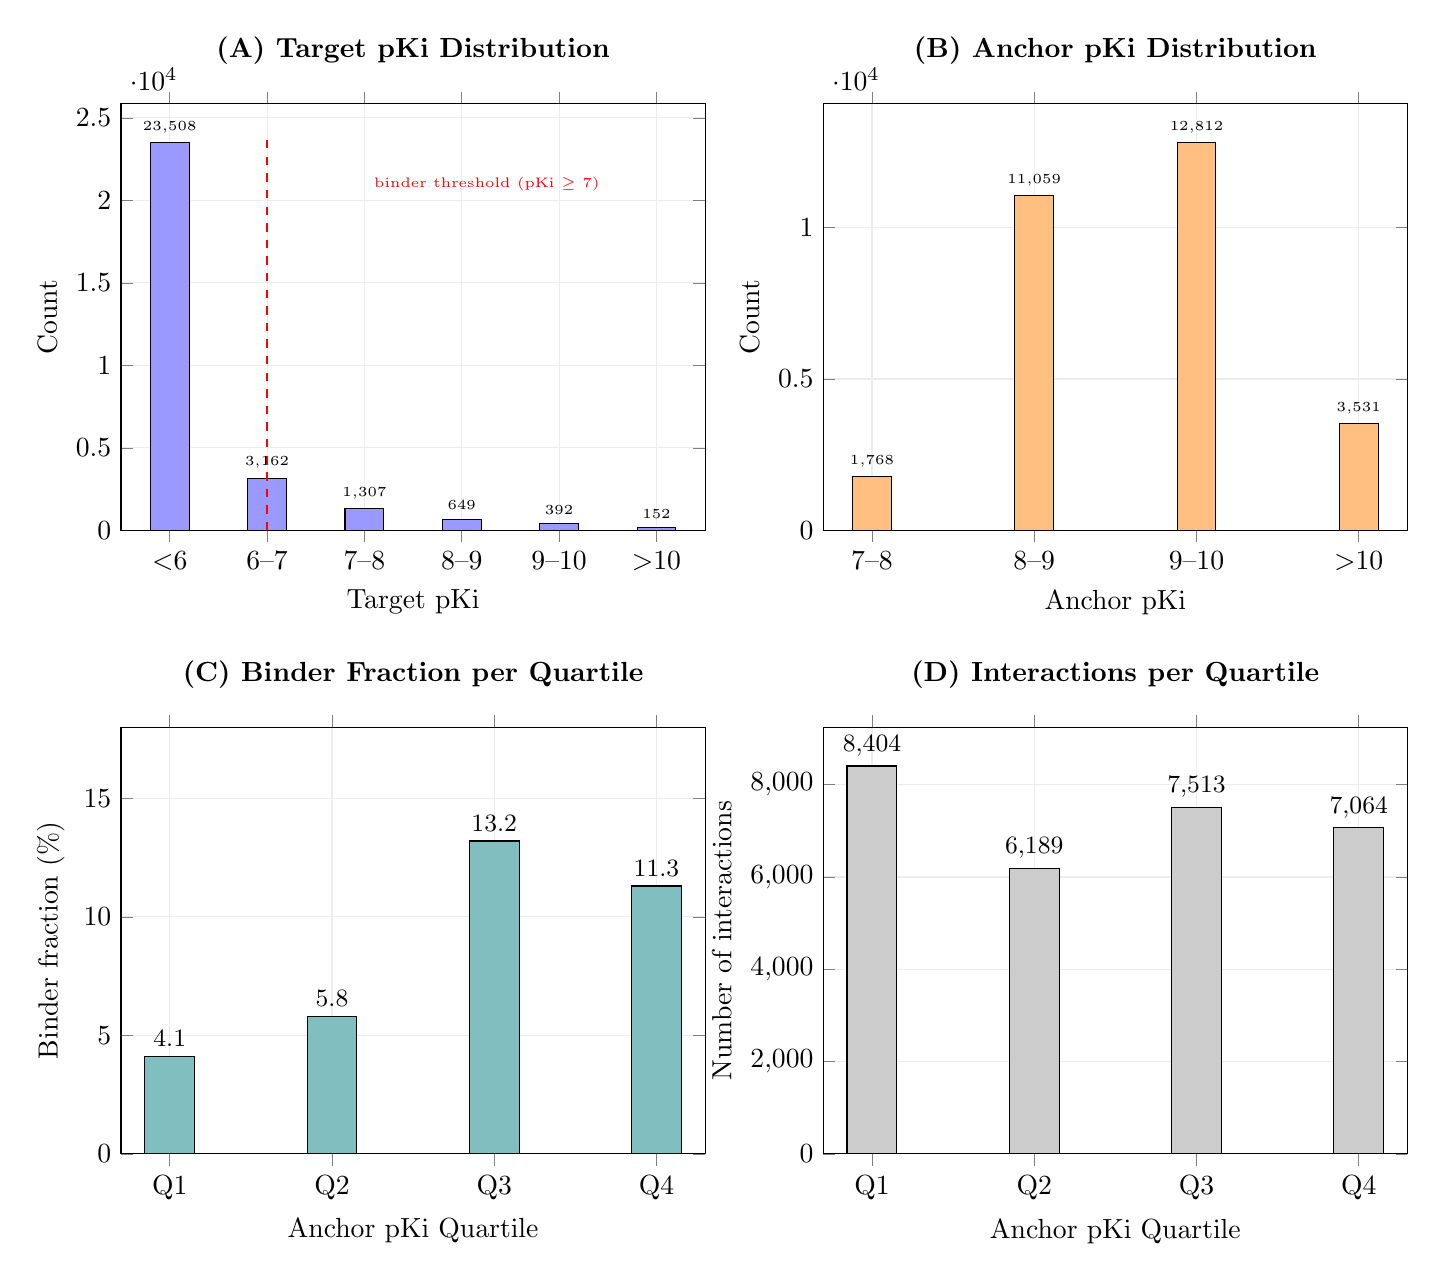
\begin{tikzpicture}

\begin{axis}[
    name=panelA,
    ybar, bar width=14pt, width=9cm, height=7cm,
    ylabel={Count}, xlabel={Target pKi},
    symbolic x coords={$<$6, 6--7, 7--8, 8--9, 9--10, $>$10},
    xtick=data, ymin=0,
    title={\textbf{(A) Target pKi Distribution}},
    title style={font=\normalsize, at={(0.5,1.03)}, anchor=south},
    grid=major, grid style={gray!15}, ymajorgrids=true,
    nodes near coords, nodes near coords style={font=\tiny, anchor=south},
]
\addplot[fill=blue!40] coordinates {
    ({$<$6}, 23508) (6--7, 3162) (7--8, 1307) (8--9, 649) (9--10, 392) ({$>$10}, 152)
};
\draw[red, dashed, thick] (axis cs:6--7, 0) -- (axis cs:6--7, 24000);
\node[red, font=\tiny, anchor=south west] at (axis cs:7--8, 20000) {binder threshold (pKi $\geq$ 7)};
\end{axis}

\begin{axis}[
    name=panelB, at={(panelA.east)}, anchor=west, xshift=1.5cm,
    ybar, bar width=14pt, width=9cm, height=7cm,
    ylabel={Count}, xlabel={Anchor pKi},
    symbolic x coords={7--8, 8--9, 9--10, $>$10},
    xtick=data, ymin=0,
    title={\textbf{(B) Anchor pKi Distribution}},
    title style={font=\normalsize, at={(0.5,1.03)}, anchor=south},
    grid=major, grid style={gray!15}, ymajorgrids=true,
    nodes near coords, nodes near coords style={font=\tiny, anchor=south},
]
\addplot[fill=orange!50] coordinates {
    (7--8, 1768) (8--9, 11059) (9--10, 12812) ({$>$10}, 3531)
};
\end{axis}

\begin{axis}[
    name=panelC, at={(panelA.south west)}, anchor=north west, yshift=-2.5cm,
    ybar, bar width=18pt, width=9cm, height=7cm,
    ylabel={Binder fraction (\%)}, xlabel={Anchor pKi Quartile},
    symbolic x coords={Q1, Q2, Q3, Q4}, xtick=data,
    ymin=0, ymax=18,
    title={\textbf{(C) Binder Fraction per Quartile}},
    title style={font=\normalsize, at={(0.5,1.03)}, anchor=south},
    grid=major, grid style={gray!15}, ymajorgrids=true,
    nodes near coords, nodes near coords style={font=\small, anchor=south},
]
\addplot[fill=teal!50] coordinates { (Q1, 4.1) (Q2, 5.8) (Q3, 13.2) (Q4, 11.3) };
\node[font=\tiny, gray, anchor=north] at (axis cs:Q1, -0.5) {[7.0--8.7]};
\node[font=\tiny, gray, anchor=north] at (axis cs:Q2, -0.5) {[8.7--9.1]};
\node[font=\tiny, gray, anchor=north] at (axis cs:Q3, -0.5) {[9.1--9.5]};
\node[font=\tiny, gray, anchor=north] at (axis cs:Q4, -0.5) {[9.6--10.8]};
\end{axis}

\begin{axis}[
    at={(panelB.south west)}, anchor=north west, yshift=-2.5cm,
    ybar, bar width=18pt, width=9cm, height=7cm,
    ylabel={Number of interactions}, xlabel={Anchor pKi Quartile},
    symbolic x coords={Q1, Q2, Q3, Q4}, xtick=data, ymin=0,
    title={\textbf{(D) Interactions per Quartile}},
    title style={font=\normalsize, at={(0.5,1.03)}, anchor=south},
    grid=major, grid style={gray!15}, ymajorgrids=true,
    nodes near coords, nodes near coords style={font=\small, anchor=south},
]
\addplot[fill=gray!40] coordinates { (Q1, 8404) (Q2, 6189) (Q3, 7513) (Q4, 7064) };
\node[font=\tiny, gray, anchor=north] at (axis cs:Q1, -200) {41 anchors};
\node[font=\tiny, gray, anchor=north] at (axis cs:Q2, -200) {23 anchors};
\node[font=\tiny, gray, anchor=north] at (axis cs:Q3, -200) {27 anchors};
\node[font=\tiny, gray, anchor=north] at (axis cs:Q4, -200) {20 anchors};
\end{axis}

\end{tikzpicture}
\end{document}
